\documentclass[12pt]{article}
\usepackage{amsmath}
\usepackage{hyperref}
\usepackage{graphicx}
\usepackage{amsfonts}
\usepackage{amssymb}
\usepackage{minted}

\usepackage{listings}
\usepackage{xcolor}
\lstset { %
    language=C++,
    basicstyle=\ttfamily,
    keywordstyle=\color{blue}\ttfamily,
    stringstyle=\color{red}\ttfamily,
    commentstyle=\color{green}\ttfamily,
    morekeywords={staple}
    morecomment=[l][\color{magenta}]{\#},
    basicstyle=\footnotesize
}

\title{Non-Perturbative QFT Problem Sheet - Question 4}
\author{Matthew Hawes}
\date{\today}


\begin{document}
\maketitle

\begin{abstract}
This question is in two sections, firstly a description of the algorithm used, followed by the results of the simulations. All code was written in c++ and is available at \url{www.github.com\\mghawes}. This was my first foray into the world of c++ so some of the implementations may not be perfect. All image rights belong to the author.
\end{abstract}

\section{Algorithm}
The algorithm, implemented in c++, relies heavily on the concept of Object-Oriented programing to improve readability as well as speed. The general principal in this case being to create objects with methods and attributes that can be initialized once and then iterated on very efficiently. The key point being that we do as much setup as possible \emph{before} beginning to perform the metropolis updates. The simplest example of this is the abstraction of the lattice into \emph{links} and \emph{staples}, which will now describe as a primer.

\subsection{Lattice}
\label{sec:lattice}
The most efficient way to store a $U(1)$ lattice is to store the phases $\theta_l$ of the group elements $U_l = \mathrm{e}^{i\theta_l}$ that live on the links $l$. In memory these links will exist as just a contiguous block, or array, of \texttt{double} values. Thus, we have to prescribe some mapping from the $2+1\mathrm{D}$ lattice to the elements of the $1\mathrm{D}$ array. The mapping chosen is to split the array into three blocks with the first third containing only $x$ directed links and the 2nd and 3rd containing $y$ and $t$ links. Within each of these blocks we `unravel' the lattice into a $1\mathrm{D}$ array by moving first along the $x$ direction, then moving along $y$ and finally along $z$. This is depicted in Fig~\ref{fig:latticeunpack} and realised by the equation displayed below.
\begin{equation}
    i = \mu n/3  +  x \, \% \, n_x + n_x \left(  y \, \% \, n_y + n_y \left( t \, \% \, n_t \right) \right)
\end{equation}
Where $i$ is the $1\mathrm{D}$ index, $\mu \in \{0,1,2\}$ is the direction of the link and $(x,y,t)$ is the location of the link in the $n=n_x\times n_y \times n_t$ lattice. Note that $\%$ represents remainder division, in order to enforce the periodic boundary conditions.\footnote{Strictly speaking this equation would fail if directly implemented into c++ code as it doesn't properly handle $x,y,t \in \mathbb{Z}^-$. This can easily be done by instead using $ (x+n_x) \% n_x$ to extend the range of validity down to $x=-n_x$}

\par With this mapping in place it is possible to obtain the value of any link specified by $(\mu,x,y,t)$ and indeed the values of the links connected to it. The neighbouring links can be accessed by incrementing the coordinates along the appropriate directions and recalculating the index. With this in place we can define our lattice as an array of link objects that each point to a different lattice value. The utility of this class based approach will become clear as we consider the implementation of the metropolis update.

%\begin{lstlisting}
%class link {
%    private:
%        double *value;		//pointer to link value
%        staple staples[4];	//array of staples
%
%    public:
%        link(double latticedata[n], std::array<int, 4> index);
%        int update(double phase,double uniformrand);
%};
%\end{lstlisting}



\begin{figure}
\centering
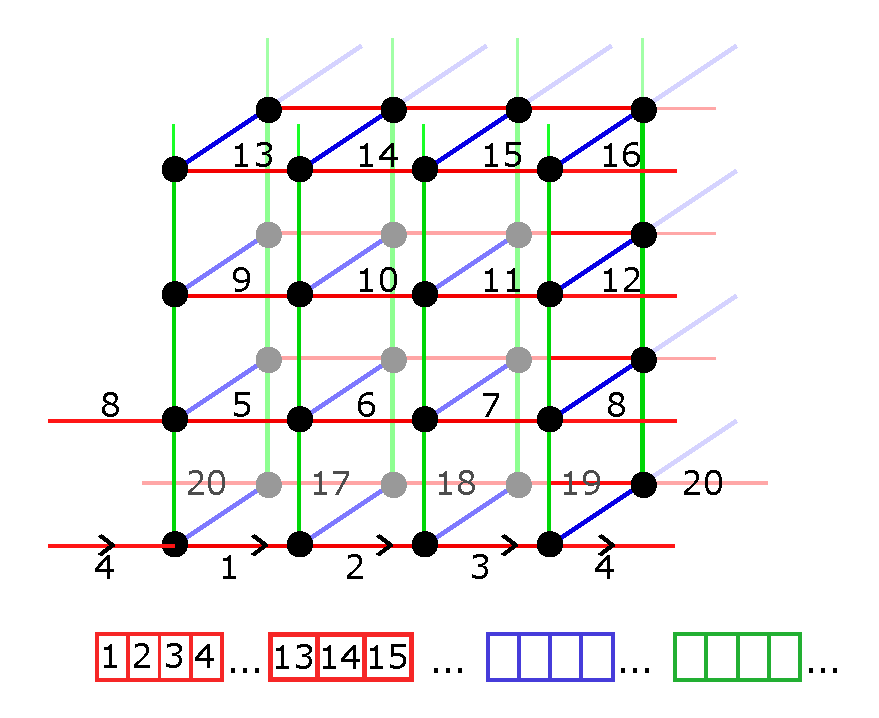
\includegraphics[width=0.6\linewidth]{latticeunpack.pdf}
\caption{'Unraveling' the links of the periodic lattice into a $1\mathrm{D}$ array depicted beneath the lattice.}
\label{fig:latticeunpack}
\end{figure}

\subsection{Metropolis}
Building on the class model of Section~\ref{sec:lattice} we can define an update method of the link class that takes a specified random phase $\theta_l'$ and attempts to update the link $U_l = \mathrm{e}^{i\theta_l}$ to this new phase. The random phase is chosen from a gaussianly distributed set of phases that is symmetric about zero and sufficiently large in order to satisfy reversibility and ergodicity. The variance of the distribution can be tuned to obtain around a 50\% update acceptance rate, this corresponds to $\sigma \approx 0.7$.

\par The randomness required by the probabilistic nature of the Metropolis algorithm is provided several pseudo-random number generators. Specifically the \emph{Mersenne Twister} algorithm, seeded with different clock values for each required random sequence. These random sequences are then mapped to different distributions, e.g, Gaussian or Uniform.

\par The uniform distribution is required for the main operation in the Metropolis update. This is the acceptance of a link update with probability 

\begin{equation}
\tilde{P}(U_l \rightarrow U_l') =  \begin{cases} 
      \mathrm{exp}\left\{-\beta \left[S(U_l')-S(U_l) \right]\right\}, & S(U_l') > S(U_l) \\    
      1, &  S(U_l') < S(U_l).
   \end{cases}
\end{equation}
Using the uniform random number $r \in [0,1)$ we can implement this acceptance by simply checking for $r<\tilde{P}(U_l \rightarrow U_l')$. This occurs when the \texttt{link::update()} method is called on a link. This method requires the \emph{change} in the action, which is where the `staples' come in. The action is defined as
\begin{align}
    \label{eq:action}
    S(\{U_l\}) &= \sum_{\{U_p\}}(1-\mathrm{Re}\{U_p\}),\\
    \mathrm{where} \; U_p &= \prod_{\{U_l\} \in U_p} U_l,
\end{align}
where $\{U_p\}$ is the set of all plaquette operators. Each $U_p$ product is formed from an ordered traversal of the square on the lattice that define the plaquette, see Fig~\ref{fig:plaq}. As our gauge field is abelian there is no issue of product ordering, however the direction of traversal for each link is important. When a link is traversed in the negative direction the conjugate field is used in the product.

\par From this definition of the action we can see that if only one link is changed then the change in the action is localised to only those plaquettes containing the changed link. Note also that the overall sense of plaquette traversal, i.e. clockwise or anticlockwise, is irrelevant as we take the real part. Thus it is convenient to define the changed link to be traversed in the forward direction, see Fig~\ref{fig:staples}. This suggest the notion of staples $\{\xi_l\}$ belonging to each link that will be required by the link during a Metropolis update. Mathematically, from \eqref{eq:action}, \begin{equation}
    \Delta S = \sum_{\{\xi_i\}} \cos(\theta_l' + \xi_i) - \cos(\theta_l + \xi_i).
\end{equation}
Where the staples $\{\xi_i\}$ are appropriately signed sums of staple phases as shown in Fig~\ref{fig:staples}.

\begin{figure}
\centering
\hspace*{-1cm}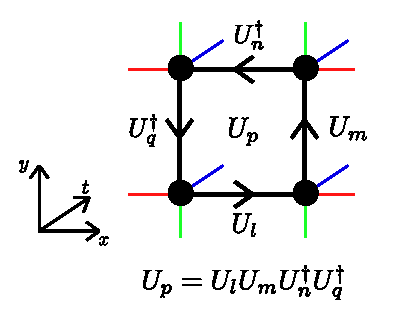
\includegraphics[width=0.5\linewidth]{plaq.pdf}
\caption{\label{fig:plaq} Pictorial representation of the plaquette operator $U_p$.}
\end{figure}

\begin{figure}
\centering
\hspace*{-1cm}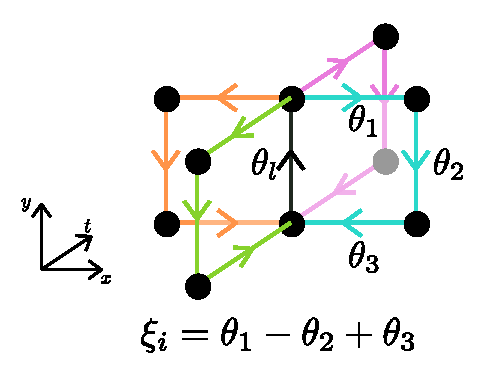
\includegraphics[width=0.5\linewidth]{staples.pdf}
\caption{\label{fig:staples} Pictorial representation of the concept of a staple. In each case the phase $\theta$ is the phase parameterising the $U$ operator that lives on the link, $U = \mathrm{e}^{i\theta}$.}
\end{figure}

\par Returning to our notion of link objects we can see that although it is possible to calculate the index of all the staple links every time we update, this is very inefficient. By defining staples as class member objects that point to links and have the appropriate signs for calculating $\xi_i$ already assigned we can economise our effort. By doing so the only operations needed to retrieve a staple value are a series of three dereferences followed by three additions.\footnote{I don't believe that there is any way of further minimising the effort of getting the link values.}

\par This class structure also provides a nice way of defining operations on the links as class methods. We also gain a degree of encapsulation, though this is not true encapsulation as multiple objects access the same links. To summarise, the diagram in Fig~\ref{fig:latticeclass} displays a simplified pictorial representation of the class structure.

\begin{figure}
\centering
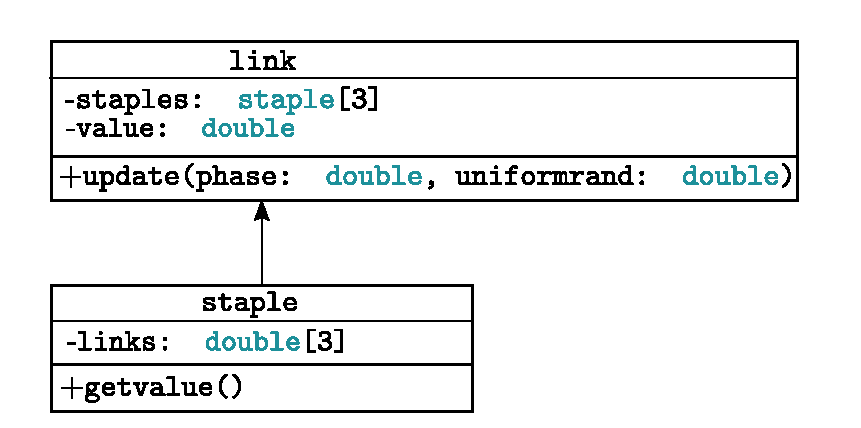
\includegraphics[width=0.7\linewidth]{latticeclass.pdf}
\caption{\label{fig:latticeclass} Simplified `UML like' class diagram of the lattice and staple classes}
\end{figure}

\subsection{Masses}
The smallest glueball masses in the theory are calculated using correlation functions $C(t)$ defined as
\begin{equation}
    C(t) = \langle \Phi(n_t)^{\dagger}\Phi(0) \rangle \underset{n_t\rightarrow \infty}{\propto} \mathrm{e}^{-amn_t}.
\end{equation}
Where the expectation is an average over field configurations generated using the Metropolis update method. The idea being to create a sequence of field configurations where each configuration differs by an update attempt on \emph{all} links, the ordering is not important. Then measure $\Phi(n_t)^{\dagger}\Phi(0)$ for each configuration and average this quantity over the sequence to get $C(t)$.

\par The two masses are the $J^{PC} = 0^{--}$ and $0^{++}$ masses, $m_{0^{--}}$ and $m_{0^{++}}$. These are calculated from the operators
\begin{align}
    \Phi_{m_{0^{++}}}(n_t) &= \sum_{\bar{n}} \left[  \mathrm{Re}\{\tilde{U}_p(\bar{n},n_t)\} - \langle \mathrm{Re}\{\tilde{U}_p\} \rangle \right]\\
    \mathrm{and} \; \Phi_{m_{0^{--}}}(n_t) &= \sum_{\bar{n}}  \mathrm{Im}\{\tilde{U}_p(\bar{n},n_t)\},
\end{align}
where $\bar{n} = (x,y)$ and the $\tilde{U}_p$ are plaquettes lying in the $xy$ plane only. The sum over all spatial sites is akin to the zero momentum fourier mode and so these operators project onto states with zero momentum. The choice of real and imaginary parts is used to pick out the desired charge conjugation symmetry. The effect of charge conjugation on a continuum gauge field is $A^{\mu} \rightarrow -A^{\mu}$. Thus, via the definition of a Wilson loop operator as
\begin{equation}
    \mathrm{Tr}\left(\mathcal{P}\exp\left(i\oint_{\gamma}A_{\mu}\mathrm{d}x^{\mu}\right)\right),
\end{equation}
this corresponds to a reversal of the path direction in the lattice theory. Forming operators that project exclusively onto either the $+$ or $-$ symmetry sectors can thus be achieved by taking Re or Im of the plaquette, as depicted in Fig~\ref{fig:reimparts}. The subtraction of $\langle \mathrm{Re}\{\tilde{U}_p\} \rangle$ in $m_{0^{++}}$ is a removal of the vacuum expectation value from the operator.

\begin{figure}
\centering
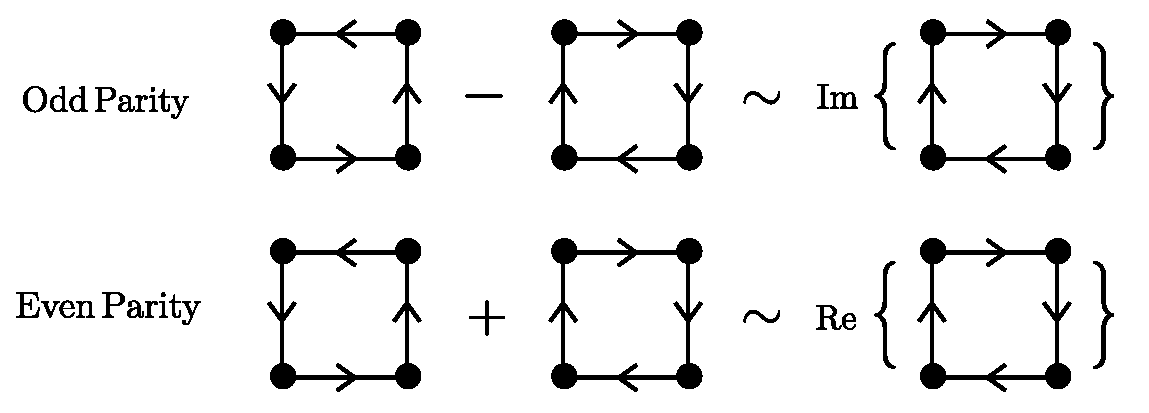
\includegraphics[width=0.8\linewidth]{reimparts.pdf}
\caption{\label{fig:reimparts} Forming operators that project onto separate symmetry sectors.}
\end{figure}


\par Following in the same vein as previously, we now consider how to abstract this operator into our object oriented picture. Each time we generate a field configuration the minimal amount of processing that must be done to measure $\Phi(n_t)^{\dagger}\Phi(0)$ for all $t$ is to obtain the link values and calculate the plaquette sum. Thus the natural object is a \texttt{twall} or \emph{T-wall} with class member \texttt{plaq} objects lying in a single constant $t$ plane. The \texttt{plaq} objects each point to the relevant four links and possess a \texttt{plaq::getvalue()} method to return $U_p$. This is depicted in Fig~\ref{fig:phiops} and Fig~\ref{fig:wallclasses}.


\begin{figure}
\centering
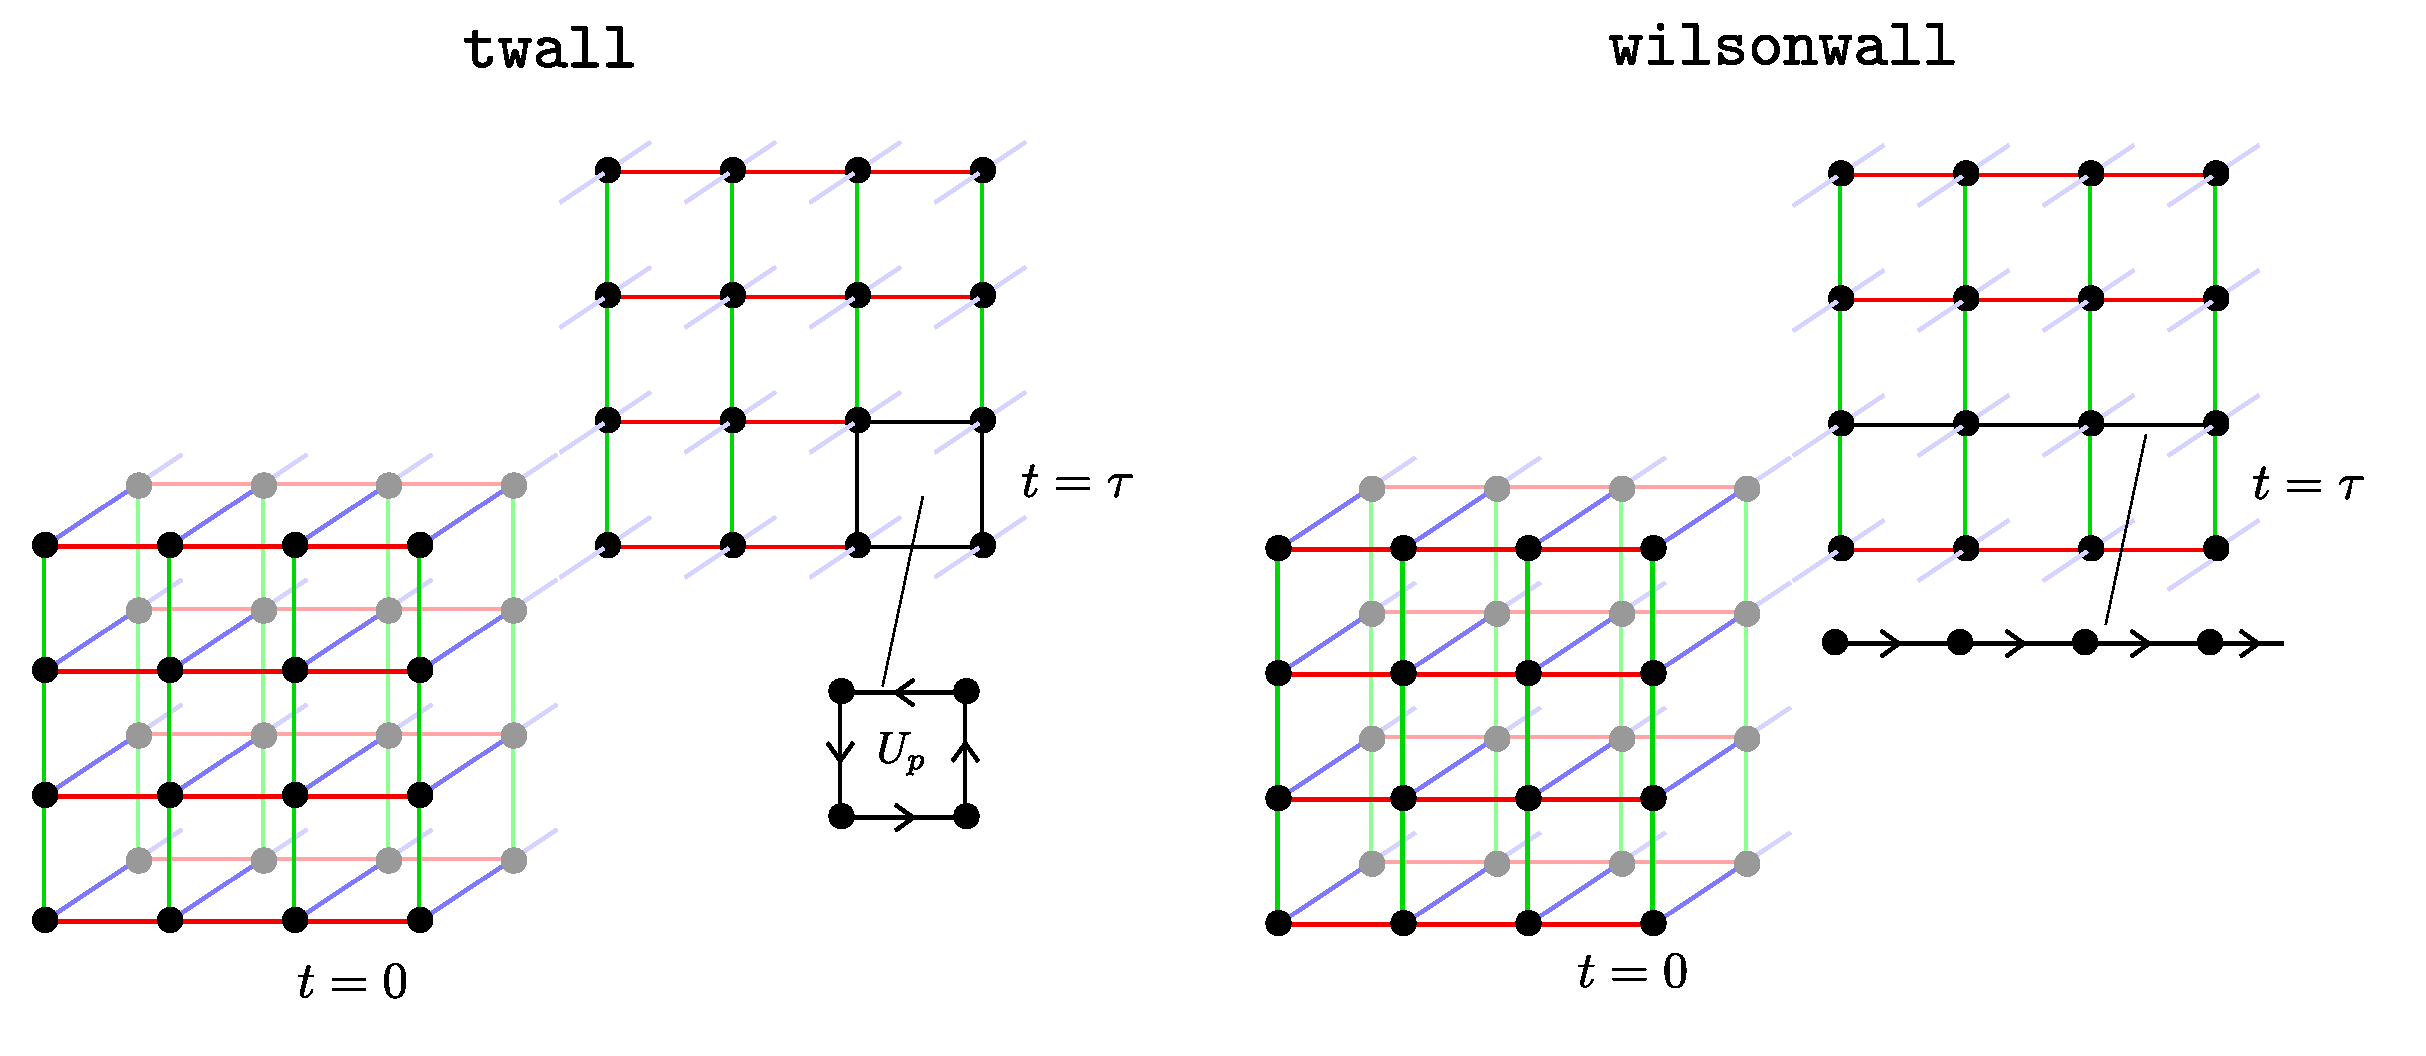
\includegraphics[width=\linewidth]{wallops.pdf}
\caption{\label{fig:phiops} Pictorial representation of the `wall' operators. Note that here the plaquettes formed at the edge of the lattice by the periodic boundary conditions are not shown.}
\end{figure}

\begin{figure}
\centering
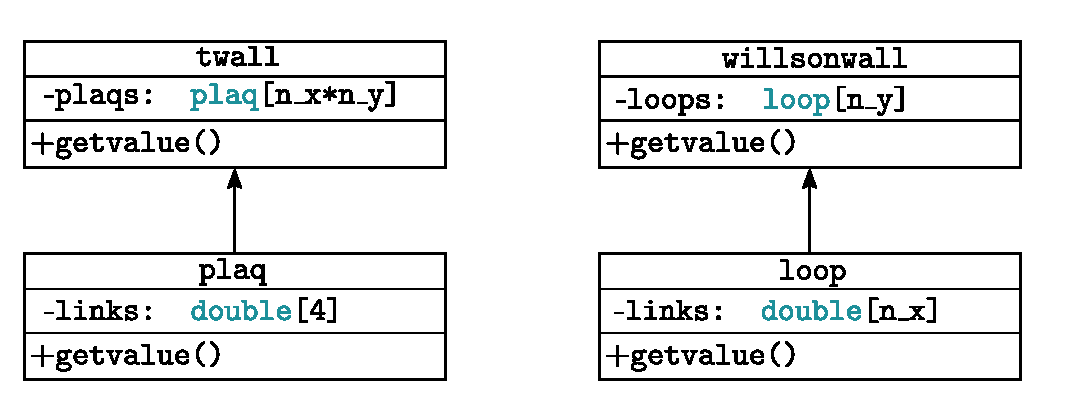
\includegraphics[width=0.8\linewidth]{wallclasses.pdf}
\caption{\label{fig:wallclasses} Simplified `UML like' class diagram of the `wall' classes}
\end{figure}

\subsection{String Tension}
The string tension is calculated similarly by considering infinite Wilson loop operators constructed from operators that wrap around the whole lattice,
\begin{align}
    \Phi_{Wilson}(n_t) &= \sum_{n_y} \prod_{n_x=1}^{n_x=L_x} U_{\hat{x}}(n_x,n_y,n_t).
\end{align}
As previously, this suggests the notion of \texttt{wilsonwall} objects defined at a given $t$, containing $L_y$ \texttt{loop} objects that each point to $L_x$ links forming a loop. This is depicted in Fig~\ref{fig:phiops} and Fig~\ref{fig:wallclasses}. The confining tension $a^2\sigma$ is calculated using the `Nambu-Goto' formula
\begin{equation}
    E_f(l = aL_x) = \sigma l\left( 1 - \frac{\pi}{3\sigma l^2} \right)^{\frac{1}{2}}.
\end{equation}
Which in the limit of large $l$ becomes
\begin{equation}
    E_f(l) \underset{l \rightarrow \infty}{=} \sigma l - \frac{\pi}{6l} + O\left(\frac{1}{l^3}\right).
    \label{eq:ng}
\end{equation}

\subsection{Code Overview}
Now that we have our principal objects of the algorithm it remains only to describe how they are pieced together. \texttt{main()} begins by setting up the relevant files for output and timers to record runtime. After this, the lattice and operator objects can be initialized and instantiated to their appropriate values. This involves using member routines to calculate where the appropriate links are and set pointers to these. For example, perform the calculation of which staples are connected to what link and where in memory those link values of the staples are actually stored.

\par After this setup we run $N_{equilib} = 20000$ Metropolis sweeps through the lattice in order to reach an equilibrium configuration. Whilst doing so we monitor the acceptance rate of link updates to ensure we are at around 50\%. Additionally we can measure the runtime and make extrapolations about the completion time. After equilibrating we can begin to make measurements, which is most easily explained in the following pseudocode. For brevity we only show the measurement of one correlator.

\begin{minted}{python}
for seq_no in range(N_sequences):
    correlatoravg = [0]*n_t
    acceptances = 0
    for fieldconfig in range(N_configs):
        for link in range(N_lattice):
            acceptances += lattice[link].update()
        for T in range(n_t):
            phi_T = twallarray[T].getvalue()
            for t in range(n_t):
                phi_tplusT = twallarray[(t+T)%n_t].getvalue()
                correlatoravg[t] += phi_tplusT*phi_T
        correlatoravg = correlatoravg/N_mes
        print('seq'+seq_n+'='correlatoravg)
\end{minted}
This code also shows how we may use the imposed periodicity of our lattice to improve the quality of our data. We do so by measuring $\Phi(t+T)\Phi(T)$ and sweeping over $T$. A great deal is absent from the above code but it gives a good idea of the skeleton of the algorithm. We have not mentioned an `average plaquette' class. This is because the ability to obtain plaquette values is built into the link and staple classes.

\par There are a few final points that deserve mention, particularly concerning runtimes and possible speed ups. I believe the class based structure gives us a good base of speed to work from. However, I do not know this for certain. I also think a lot of it will come down to compiler implementation, which is a bit too low level for a virginal c++ programmer. Despite this, one obvious significant speedup is that of parallelisation, which for this algorithm is trivial to implement. One can simply run multiple instances of the code, started at slightly staggered times so as to obtain different clock times for the random seed. In this way we are simply multi-processing and there is no complication of thread-safety, as with multi-threading. Upon completion is then the small matter of amalgamating the data outputs. Table~\ref{tab:runtimes} displays the average runtimes for all lattice sizes.

\begin{table}[h]
  \centering
    \begin{tabular}{l|c|c|c}
Lattice Size & $18\times 18 \times 24$ & $22\times 22\times 36$ & $28\times 28\times 40$ \\ \hline
Runtime (hrs:mins)         & 0:52     & 1:33     & 2:57  \\

\end{tabular}
\caption{Total runtimes for calculations at a \emph{single} $\beta$ parallelised into 5 processes. Each process outputs 6 subsequences of 10000 field configurations each, giving us 30 sequences in total. This includes Metropolis update time and time taken to make measurements.}
\label{tab:runtimes}
\end{table}

Putting this all together means that the total runtime for all $\beta=2.0,2.1,2.2,2.3$ on all lattices falls in at just less than a day of computing time. Which I'm actually rather pleased with!



\section{Results}
At this point our simulations have produced files containing the four desired quantities for different values of $\beta$ on different lattice sizes. As stated previously, the field configurations used were split at runtime into $n=30$ subsequences so as to obtain error estimates for the various values. We begin by describing the process of calculating these error estimates, all of which was implemented in python because it's much easier than c++!

\subsection{Errors\protect\footnote{My understanding of statistics is perhaps not as good as it ought to be and as you will see I have a couple of cautious concerns about what I've done in this section.}}
Each subsequence gives us a measurement `$x_i$' for each of our `quantities', for example $C_{m_{0^{++}}}(t=4)$ on $28\times 28 \times 40$ at $\beta = 2.2$. Thus we can use unbiased estimators to form data points with errors
\begin{align}
    \bar{x} &= \frac{1}{n}\sum_{i} x_i,\\
    \bar{\sigma}_{x}^2 &= \frac{1}{n-1}\sum_{i} (x_i - \bar{x})^2.
\end{align}
We do not know the underlying distribution's standard deviation, in fact we don't know its distribution at all! However, given that the $x_i$ measurements themselves are in fact an arithmetic mean over $N=10000$ field configurations we may use the central limit theorem to say that the $x_i$ are in fact Gaussianly distributed. There is a point of contention here about the fact that the central limit theorem requires the sum of \emph{independent} random variables. Strictly speaking the field configurations are certainly not independent as they are generated from each other in sequence. Thus we would fully expect there to be some correlation, but I imagine it is probably not so relevant given the sufficiently large $n$ and perhaps some appeal to ergodicity. Moving on\ldots

\par When sampling from a Gaussian distribution with unknown standard deviation we must use the t-distribution for our standard errors.
\begin{equation}
x = \bar{x} \pm t_{n,\alpha} \frac{\sigma_x}{\sqrt{n}}
\end{equation}
Where this specifies the error for a $(1-\alpha)\times100\%$ confidence interval, in this case I chose the seemingly standard $95\%$ interval. The value of $t_{n,\alpha}$ is chosen from t-distribution tables. Before we completely discard all information about our $n$ field configurations it is good to first check that our assumption of no correlations between simulations is indeed valid and that our residuals are random. The plot in Fig~\ref{fig:residuals} suggests we are correct in our assumption of no inter-sequence correlation. This obviously doesn't violate the presence of intra-sequence correlation.

\begin{figure}
\centering
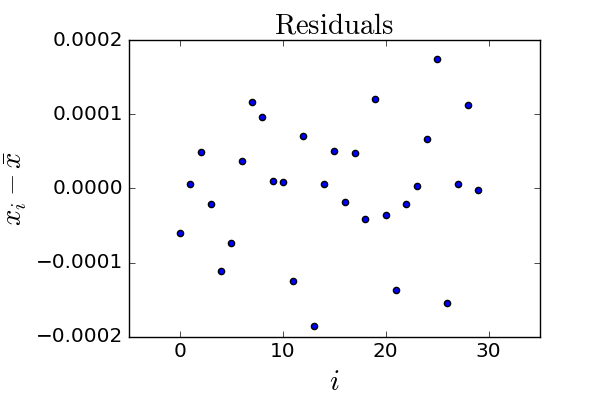
\includegraphics[width=0.6\linewidth]{residuals.png}
\caption{\label{fig:residuals} }
\end{figure}


\subsection{Fitting}
Now that we have standard errors on all our measurements it is possible to fit our results. Obviously this is only necessary for our correlators $C(t)$ satisfying $C(t) \underset{t\rightarrow \infty}= c\mathrm{e}^{-aEn_t}$ and not the average plaquette.

\par All fitting and further analysis was performed in OriginPro. We expect to see some discrepancy between the data and the fits for various reasons, including finite size effects and inherent fluctuations from the Monte Carlo approach. Figure~\ref{fig:massfitting} displays the fitting process for the $m_{0^{--}}$ and $m_{0^{++}}$ masses. In each case the decision was made to fit the curves to either

\begin{align}
    y &= a\mathrm{e}^{bx},\\
    \mathrm{or} \; \; y &= y_0 + A\mathrm{e}^{R_0x}.
\end{align}

\begin{figure}
  \centering
  \begin{minipage}[c]{\linewidth}
    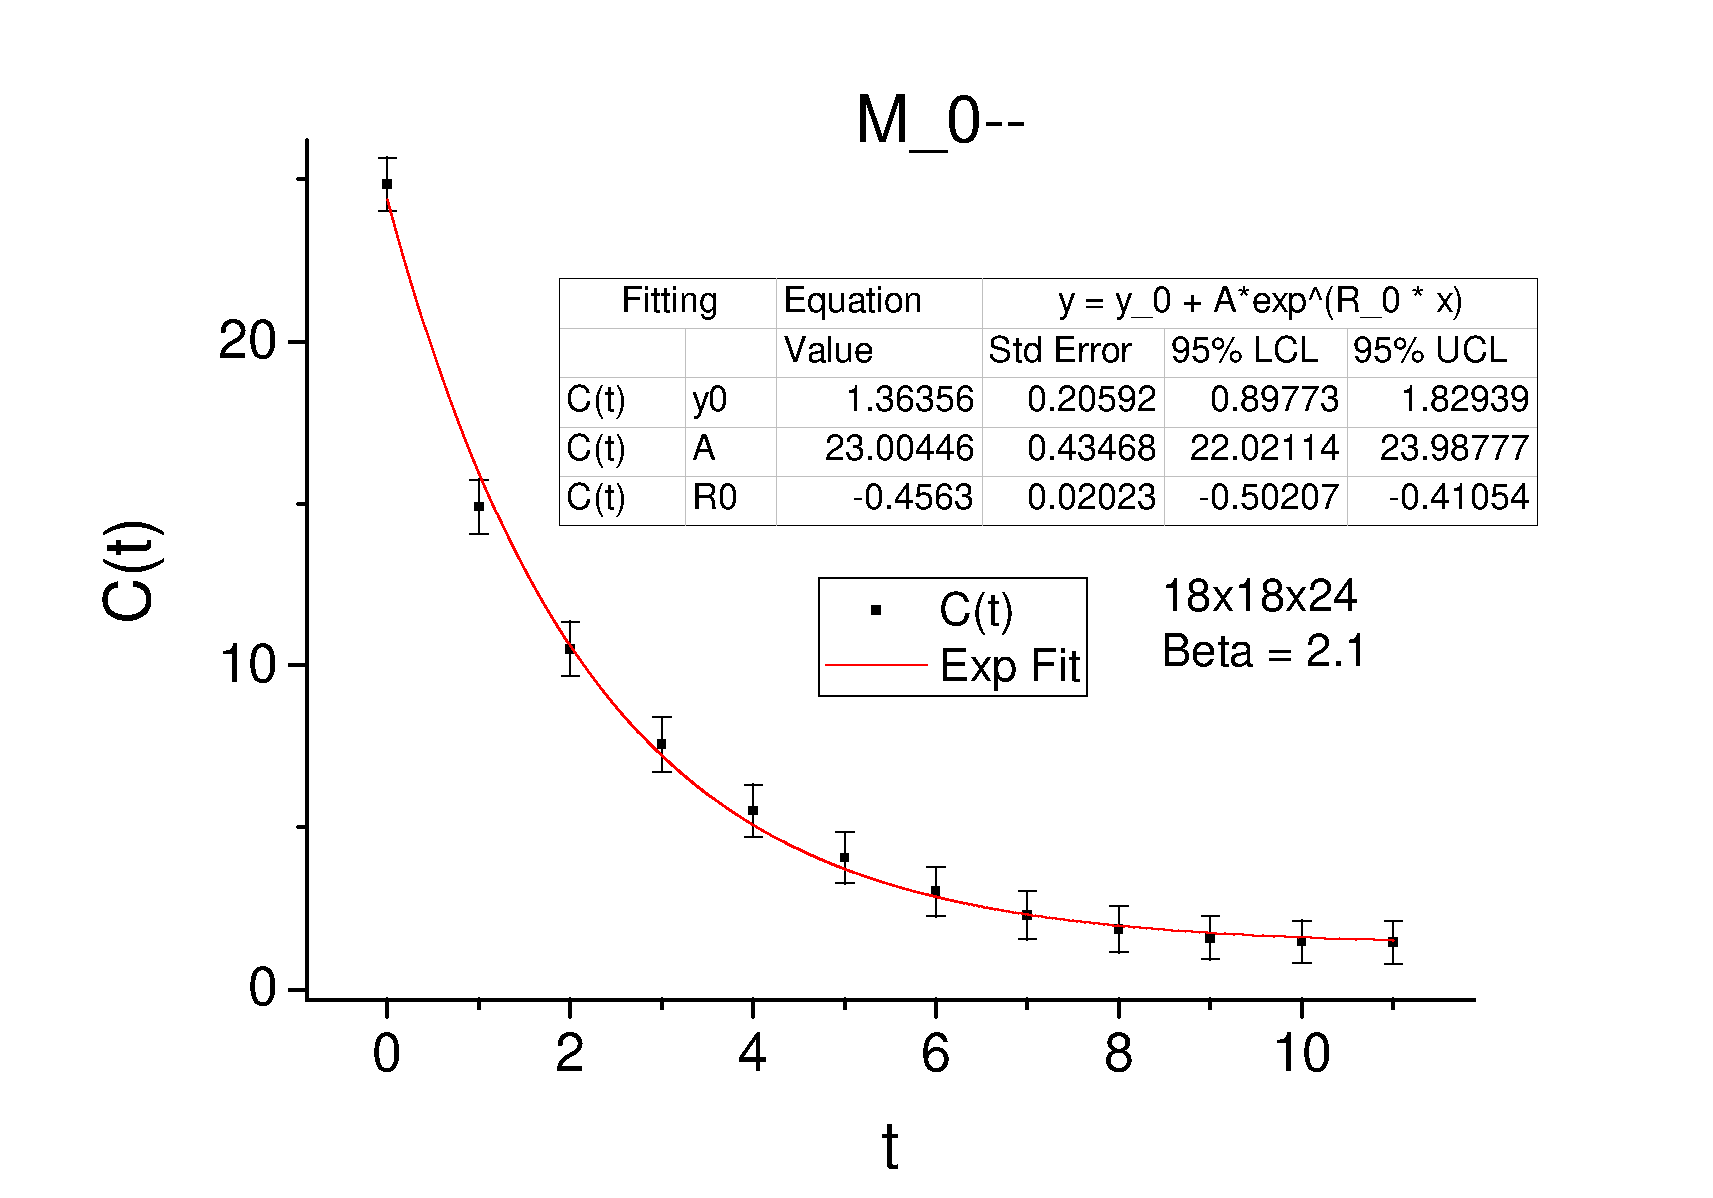
\includegraphics[width=\linewidth]{m--fit.pdf}
  \end{minipage}
  \begin{minipage}[c]{\linewidth}
    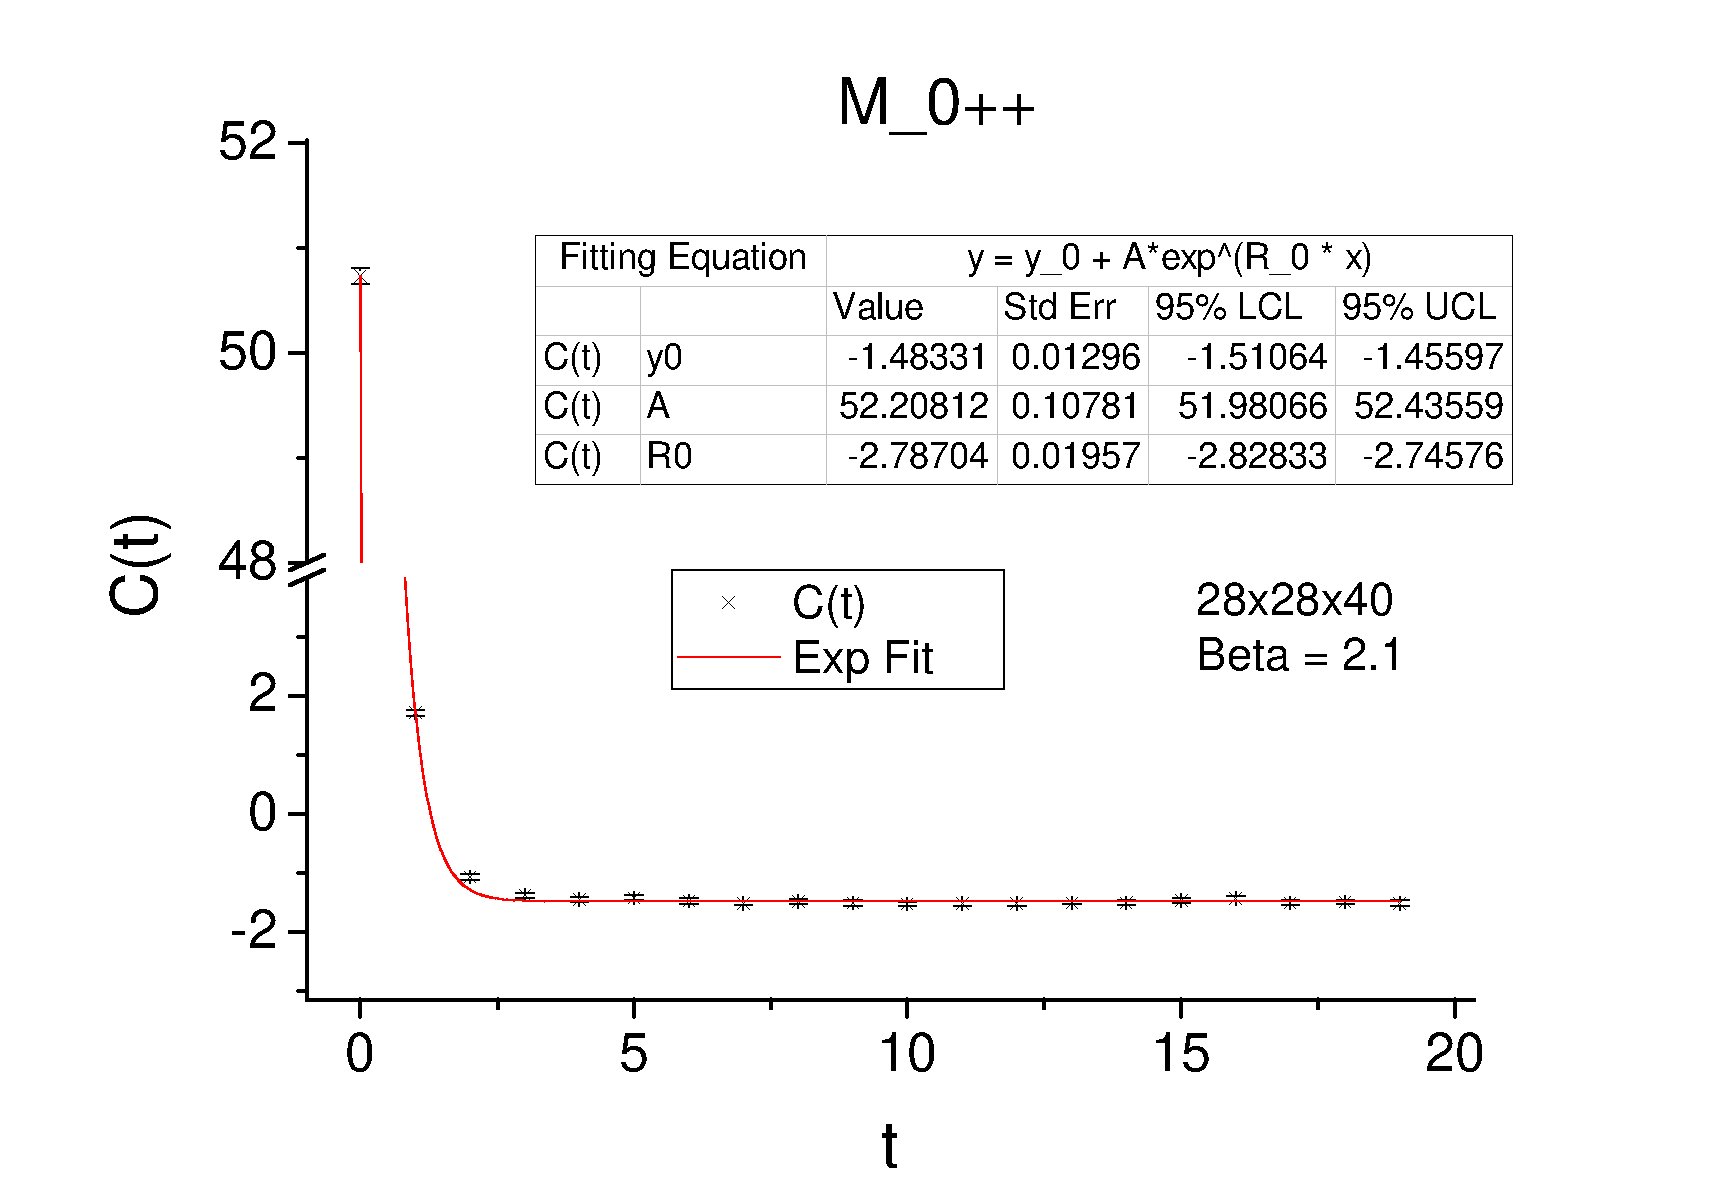
\includegraphics[width=\linewidth]{m++fit.pdf}
  \end{minipage}
\caption{Masses exponential fitting.}
\label{fig:massfitting}
\end{figure}


The offset was chosen as some of the smaller lattices especially displayed an offset that I assume is due to the aforementioned finite size. This is the reason for not just taking the logarithm and fitting that linearly.

\par As a result of the imposed periodic boundary conditions it is only valid to fit to the first half of the lattice.\footnote{I suppose you could fit both halves separately and then combine them to decrease the error but as the correlators are symmetric in I wondered if this would constitute an over fitting of the data.}

Figure~\ref{fig:massfitting} shows exceptionally tight error bars for the $m_{0^{++}}$ and the same is true of the Wilson loops. This is present in all lattice sizes at all $\beta$ which is somewhat concerning, but the fits seem good? Once again, moving on\ldots

\par After applying this fitting process to all simulations we obtain the value of `$E$' for each of our correlators. In the case of the masses this is exactly what was required to be calculated and the results are listed in Table~\ref{tab:massfitting}. The tables list the value of $m_{0^{--}}$, $m_{0^{++}}$, and the average plaquette as this has been available for a while. The errors listed here are the 95\% confidence interval bounds for the fitting parameters, determined by Origin. This calculation takes into account the errors on the individual points. The fitting routine itself also makes use of the error bars, using them inversely as weights in the fitting.


\begin{table}
  \centering
  \begin{minipage}[c]{\linewidth}
  \centering
    \begin{tabular}{l|c|c|c}
$m_{0^{++}}$ & $18\times 18 \times 24$ & $22\times 22\times 36$ & $28\times 28\times 40$ \\ \hline
2.0          & 2.680 $\pm$ 0.085       & 2.690 $\pm$ 0.112     & 2.666 $\pm$  0.050  \\
2.1          & 2.790 $\pm$ 0.061       & 2.785 $\pm$ 0.045     & 2.787 $\pm$  0.041  \\
2.2          & 2.880 $\pm$ 0.079       & 2.874 $\pm$ 0.053     & 2.875 $\pm$ 0.045  \\
2.3          & 2.978 $\pm$ 0.050       & 2.974 $\pm$ 0.060     & 2.976 $\pm$  0.029   
\end{tabular}
  \end{minipage}
  \newline
\vspace*{0.5 cm}
\newline
  \begin{minipage}[c]{\linewidth}
  \centering
    \begin{tabular}{l|c|c|c}
$m_{0^{--}}$ & $18\times 18 \times 24$ & $22\times 22\times 36$ & $28\times 28\times 40$ \\ \hline
2.0          & 0.546 $\pm$ 0.040  & 0.448 $\pm$ 0.038  & 0.550 $\pm$ 0.025   \\
2.1          & 0.456 $\pm$ 0.046  & 0.385 $\pm$ 0.032  & 0.378 $\pm$ 0.026   \\
2.2          & 0.392 $\pm$ 0.051  & 0.289 $\pm$ 0.029  & 0.0326 $\pm$ 0.026   \\
2.3          & 0.352 $\pm$ 0.056  & 0.272 $\pm$ 0.031  & 0.267 $\pm$ 0.023  
\end{tabular}
  \end{minipage}
  \newline
\vspace*{0.5 cm}
\newline
  \begin{minipage}[c]{\linewidth}
  \centering
    \begin{tabular}{l|c|c|c}
Avg. Plaq. & $18\times 18 \times 24$ & $22\times 22\times 36$ & $28\times 28\times 40$ \\ \hline
2.0         &   0.80594 $\pm$ 7.3e-5  &  0.81256 $\pm$ 0.005   & 0.80599 $\pm$ 3.5e-5 \\
2.1         &   0.81878 $\pm$ 5.8e-5  &  0.81876 $\pm$ 4.3e-5  & 0.81875 $\pm$ 3.9e-5 \\
2.2         &   0.82955 $\pm$ 6.1e-5  &  0.82949 $\pm$ 4.7e-5  & 0.82948 $\pm$ 3.5e-5 \\
2.3         &   0.83873 $\pm$ 6.8e-5  &  0.83868 $\pm$ 3.7e-5  & 0.83850 $\pm$ 3.2e-5 
\end{tabular}
  \end{minipage}
\caption{Mass data from fits}
\label{tab:massfitting}
\end{table}


\subsection{Further Analysis}
Although the values of the masses are obtainable directly from the exponent we must use the aforementioned Nambu-Goto formula \eqref{eq:ng} to obtain the string tension. This is done very similarly to the previous fitting, only this time linear. Figure~\ref{fig:stringtension} displays the fitting process and Table~\ref{tab:string} displayed the results and their errors. Again these errors are the 95\% confidence interval bounds for the fit parameters.

\begin{table}
  \centering
    \begin{tabular}{l|c}
$\beta$ &  String Tension \\ \hline
2.0         &   0.191 $\pm$ 0.041 \\
2.1         &   0.183 $\pm$ 0.058 \\
2.2         &   0.176 $\pm$ 0.022 \\
2.3         &   0.168 $\pm$ 0.002 
\end{tabular}
\caption{String tensions for different $\beta$.}
\label{tab:string}
\end{table}

\begin{figure}
\centering
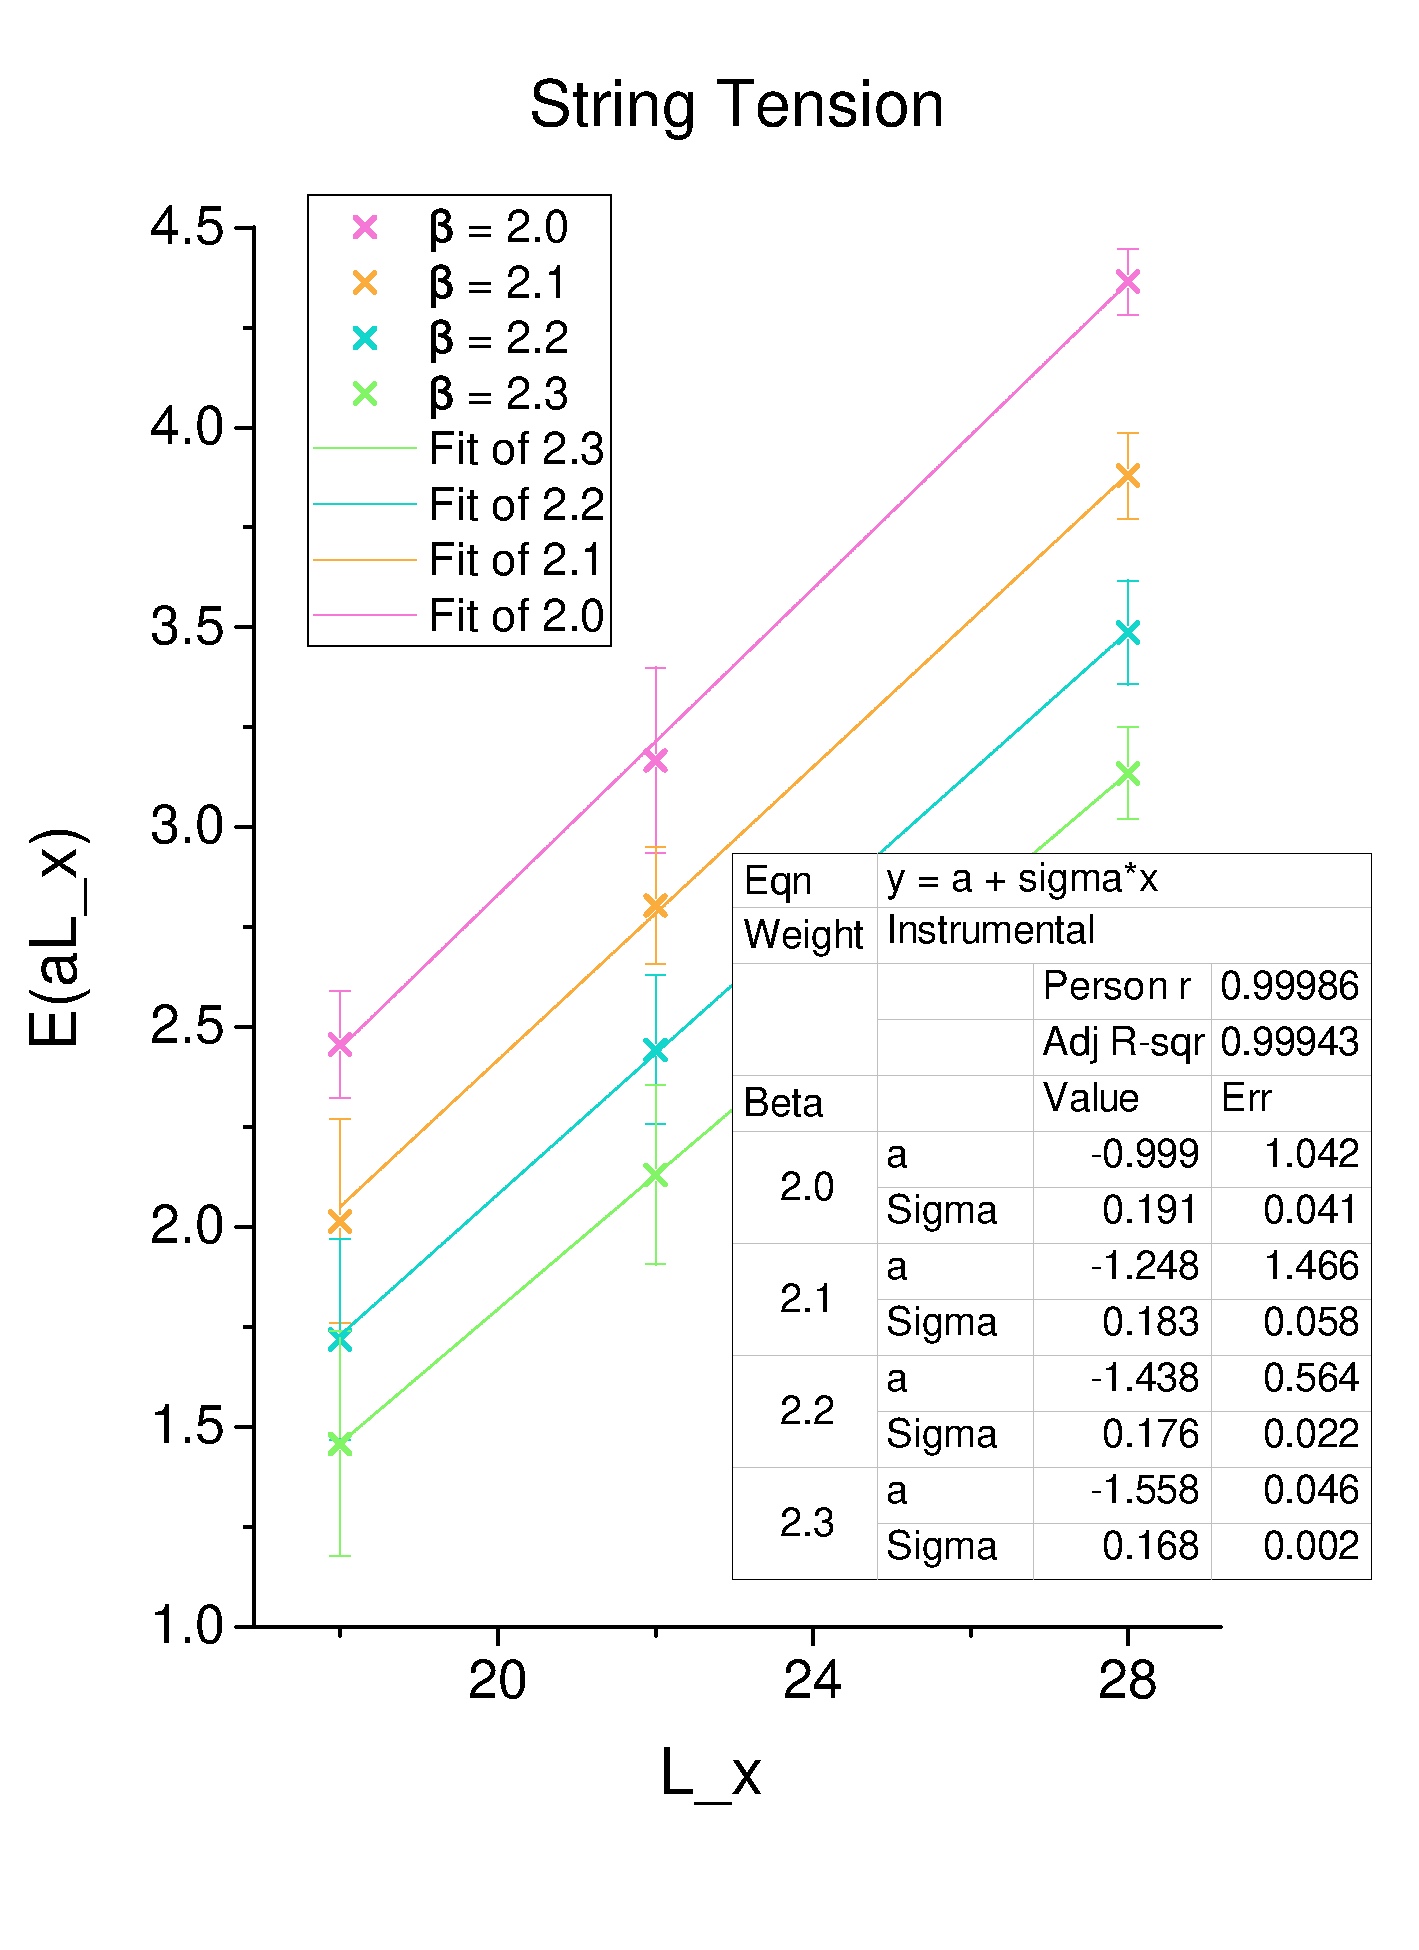
\includegraphics[width=0.8\linewidth]{stringtension.pdf}
\caption{\label{fig:stringtension} Wilson loop correlator data used to calculate the string tension $\sigma a^2$ via the Nambu-Goto formula \eqref{eq:ng}}
\end{figure}

\par Though technically we are now done we conclude by taking a look at the beta dependence of the masses in Fig~\ref{fig:betadepen}.

\begin{figure}
\centering
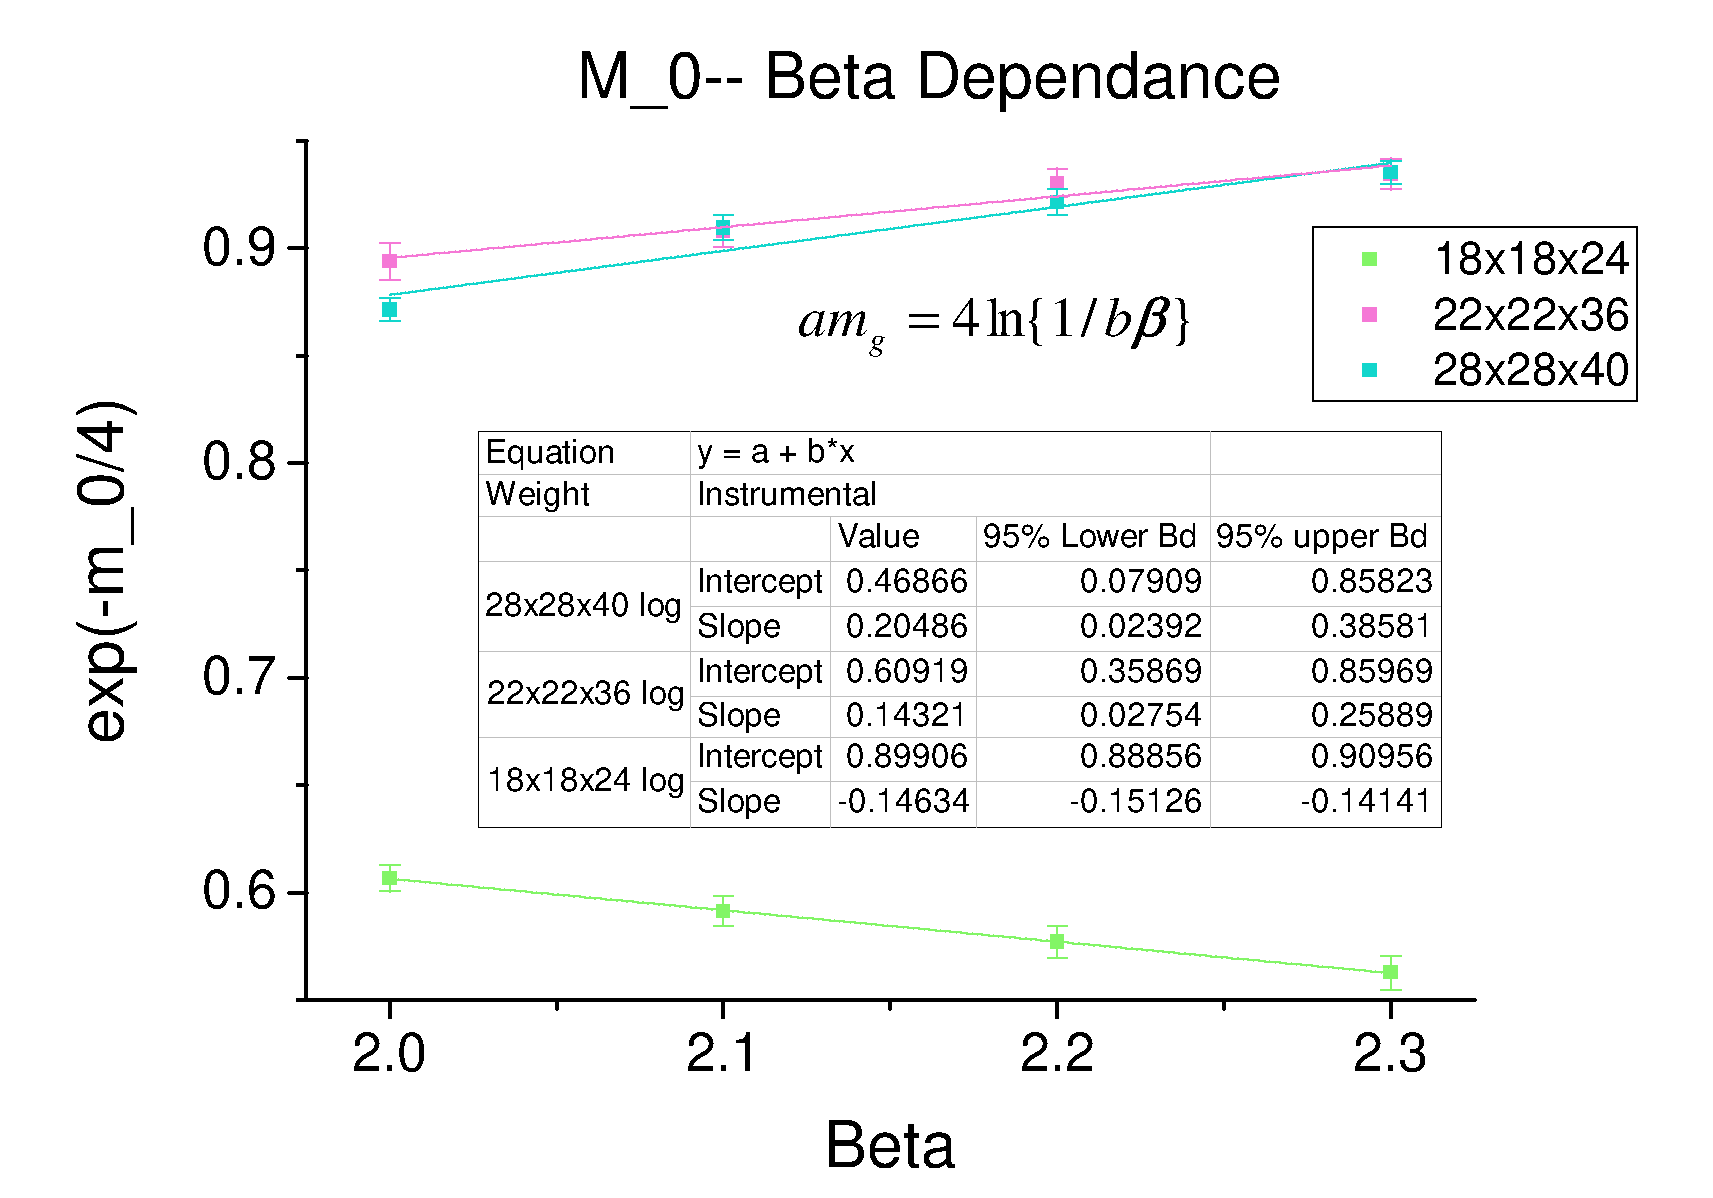
\includegraphics[width=\linewidth]{massesdepen.pdf}
\caption{\label{fig:betadepen} $\beta$ dependences of the masses for different lattice sizes. Masses are first exponentiated so that we can linear fit to $am_g = 4\mathrm{ln}(1/b\beta)$. The fits are nicely linear but a zero intercept falls just outside the 95\% confidence limits, especially for the smaller lattices.}
\end{figure}

\end{document}